\documentclass[tikz,border=1mm]{standalone}
\usepackage{pgfplots}
\usetikzlibrary{decorations.pathreplacing,calligraphy}

\begin{document}
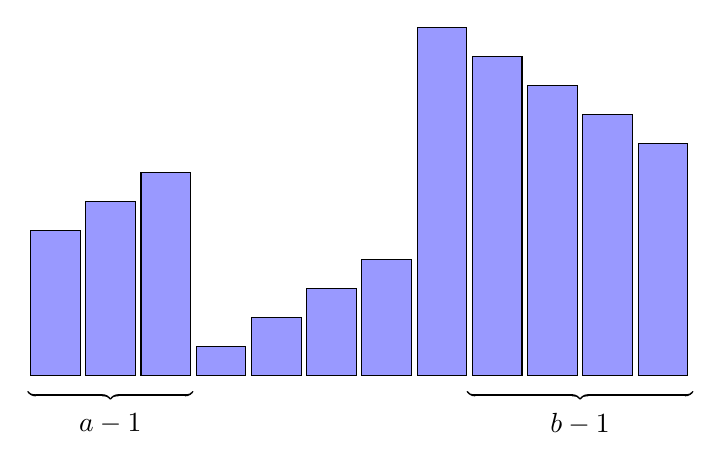
\begin{tikzpicture}

% Plot the histogram
\begin{axis}[
    ybar,
    bar width=0.63cm,
    xmin=0,
    xmax=12,
    ymin=0,
    ymax=12,
    xticklabel={\pgfmathparse{int(\tick)}\pgfmathresult},
    axis lines=none,
    axis line style={-},
	width=10cm,
	height=6cm,
]
\addplot[fill=blue!40] table {
    x y
    0.5 5
    1.5 6
    2.5 7
    3.5 1
    4.5 2
    5.5 3
    6.5 4
    7.5 12
    8.5 11
    9.5 10
    10.5 9
    11.5 8
};
\end{axis}

\begin{scope}[decoration={calligraphic brace, amplitude=1mm}]
  \draw[thick,decorate] (2.1,-0.2) -- (0,-0.2)
    node[midway,below=1ex]{$a-1$};
  \draw[thick,decorate] (8.45,-0.2) -- (5.58,-0.2)
    node[midway,below=1ex]{$b-1$};
\end{scope}

\end{tikzpicture}
\end{document}

